\section{Einleitung}

Der heutige Netzwerkverkehr ist fast tausendfach größer als vor 20 Jahre \citep{Roser_I}. Das Internet wird heutzutage für fast alle unsere alltägliche Tätigkeit verwendet:  Sozialenetzwerke, Video und Audio-Streaming, Einkauf, behördliche Angelegenheit und viele andere. So viel Verkehr generiert eine unermessliche Menge von Daten, die alle mögliche Inhalte beinhalten, von unschuldigen Anfragen nach dem eigenen Kontostand bis zu der Ausführung von bösewichten Anfragen, um Systemen lahmzumachen. Um das erste von der zweiten zu Unterscheiden verwenden vielen Firmen die sogennanten \glsfirst*{SIEM}.

Die \glsfirst{NIST} definiert \acrshort{SIEM} als Anwendung, die dafür zustäntig ist, Sicherheitsdaten von anderen Systemen zu sammeln und diese verständlich und lesbar als Information zu liefern. Mit diesem Ergebnis können Aktionen und durchgeführt werden können \citep{NIST_SIEM}. Die Bewertung dieser Daten spielt eine wesentliche Rolle bei solchen Anwendungen, da es entscheidend ist, ob es um eine oder viele normale Anfrage oder um einen \gls{Cyberangriff} geht.

In diesem Projekt wollen wir über eine existierende \gls{Open Source} \gls{SIEM}-Anwendung recherchieren und ihre Extrahierung und Bewertung von Daten analysieren. Am Ende wollen wir uns für eine der gefundenen Lösung entscheiden, sodass spezifische Logdateien bewertet und bearbeitet werden können.

Diese Arbeit wird in folgende Teile geteilt:

% OSSIN: https://sourceforge.net/projects/os-sim/
% Preludes: https://www.prelude-siem.org/projects/prelude/wiki/ManualUser
% ELK Stack

% Grafana / Promtail: https://grafana.com/products/enterprise/
%https://grafana.com/logs/% 

%https://www.ossec.net/         https://github.com/ossec/ossec-rules

% was machen sie konkrent? / Vergleich zwischen OpenSource/Proprietary/

\begin{itemize}[noitemsep]
   \item Beschreibung von existierenden \glspl{SIEM} und Vergleich zwischen privaten Anbieter und eine \gls{Open Source} Lösungen (Alienvault OSSIN, OpenSearch, MozDef, Wazuh, Preludes)
   \item Analyse der Funktionalität einer \gls{Open Source} \gls{SIEM}
   \item Definition von zwei spezifische \glsplural{Cyberangriff}
   \item Empfang und Bearbeitung der Daten von den vorher beschriebenen Angriffe
   \item Entwicklung einer Regel für die Erkennung eines \gls{Cyberangriff}
   \item Analyse und Bewertung der Arbeit
\end{itemize}

Das folgende Diagramm stellt den Aufbau dieser Arbeit dar:

\begin{figure}[H]
   \centering
   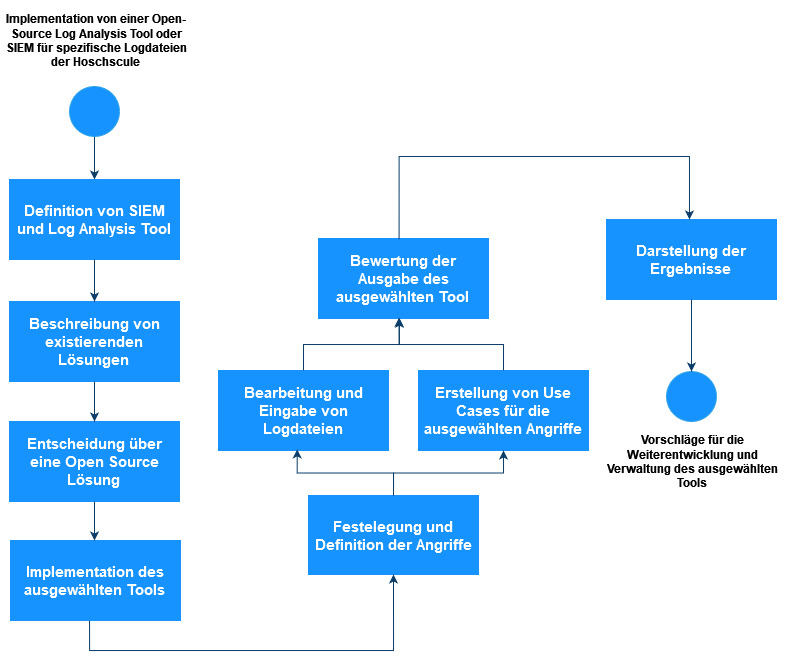
\includegraphics[width=0.8\textwidth]{assets/1_p1.jpg}
   \caption{Aufbau dieser wissenschaftlichen Recherche \gls{SIEM} \\Quelle: Eigene Darstellung }
   \centering
\end{figure}


\subsection{Problemstellung}
Während der Entwicklung dieser Arbeit wollen wir uns mit folgenden Fragen beschäftigen:

\begin{itemize}
   \item Welche Information-Muster muss von dem \gls{SIEM} extrahiert werden, um Angriff\_1 und Angriff\_2 zu erkennen?
   \item Wie sollen aussagenkräftige Use-Cases / Regel sein, um Angriff\_2 und Angriff\_2 richtig zu erkennen zu erkennen?
   \item Wie sollen Server-Logs aussehen, damit sie von \glsplural{SIEM} bearbeiten werden können.
\end{itemize}

Note: Für Angriffe habe ich an DoS und Brute-Force (Password Spraying/Dictionary) gedacht.

Note 2: Punkt 3 wäre eher theoretisch, um zu recherchieren, was es schon gibt und was schon darüber geschrieben wurde.

\subsection{Vorgehensweise}
Um diese obengenannten Ziele zu erreichen, verwenden wir folgenden Methode:

\begin{itemize}[noitemsep]
   \item Installation von virtuellen Maschinen zur Nutzung von der ausgewählten \gls{SIEM} und zur Generierung von Server-Logs
   \item Nutzung von Container zur Installation von \gls{SIEM}
\end{itemize}

